\chapter{Implementacion}
\label{chapter:implementation}

El siguiente conjunto de secciones describen la implementacion del metodo
propuesto segun las explicaciones presentadas en el Capitulo
\ref{chapter:proposed-method}. La implementacion propuesta utiliza un software
de simulacion como el mostrado en \cite{} (\url{}), este software de simulacion esta
programado en Unity con codigo fuente en lenguaje C\# de Visual Studio.

\section{Codificando los diccionarios de piezas}
\label{section:piece_dictionary}

La primera parte que se desarrollo para poder integrar el listado de piezas al
sistema de generacion fue decir la manera en como se establecerian las
diferentes piezas como las mostradas en la figura \ref{figure:game-basic-blocks}
del Capitulo \ref{chapter:proposed-method}, para esto se tomaron enncuenta
varias posibilidades, la primera, como se explica en la seccion
\ref{subsection:objectorientedidea} se buscaba ordenar las diferentes piezas
como diccionarios que contuvieran una o mas referencias a las piezas que
integraban cada entrada del diccionario, para esto las primeras 11 posiciones
eran elementos individuales uno para cada pieza como el mostrado en la figura
\ref{code:dic_individual_piece}, en el codigo se aprecia la manera en como se
designaba una pieza del juego, para poder trabajar de manera dinamica para poder
agregar mas compuestos segun fuese necesario se utilizaban dos diccionarios
extra, estos contenian los datos de los tipos de materiales posibles y la
informacion de los tamaños de las piezas, de esta manera en caso de tener mas de
una pieza en algun punto del diccionario era posible modificar el valor de
offset de cada una de las piezas calculando la distancia del punto central de
cada pieza al centro de todo el conjunto.

\begin{listing}[t]
  \begin{minted}[frame=lines, framesep=2mm,baselinestretch=1.2,fontsize=\footnotesize,linenos]{python}
    BLOCKS = {
      0: [
          {'type': BLOCK_TYPE['Circle'],
          'material': BLOCK_MATERIAL['wood'],
          'offset': [0, 0, 0] # x, y, z - Calculated from the center of the figure
          }]
    }

    BLOCK_TYPE = {
    'Circle': {'height': 72, 'lenght': 72},
    'RectTiny': {'height': 22, 'lenght': 42},
    'RectSmall': {'height': 22, 'lenght': 42},
    'RectBig': {'height': 22, 'lenght': 42},
    'RectMedium': {'height': 22, 'lenght': 42},
    'RectFat': {'height': 42, 'lenght': 82},
    'SquareTiny': {'height': 22, 'lenght': 22},
    'SquareSmall': {'height': 42, 'lenght': 42},
    'Triangle': {'height': 72, 'lenght': 72},
    'TriangleHole': {'height': 82, 'lenght': 82},
    'SquareHole': {'height': 82, 'lenght': 82}
    }

    BLOCK_MATERIAL = {
        'wood': 0,
        'stone': 1,
        'ice': 2
    }
  \end{minted}
  \caption{Ejemplo de diccionario con un solo elemento}
  \label{code:dic_individual_piece}
\end{listing}

De esta manera como se explico anteriormente era mas sencillo crear compuestos,
sin embargo, la desventaja que conyevaba utilizar este metodo era que no podiar
realizar modificaciones a las restricciones de las piezas, es decir, en caso de
querer evitar que un conjunto de piezas con determinados materiales no fuesen
generados no se tenia la facilidad de impedir este tipo de combinaciones.

En luz de esta informacion se opto por utilizar el metodo en base a clases
mencionado en la seccion \ref{subsection:classorientedidea}, el codigo
\ref{code:dic_individual_piece} muestra la nueva estructura utilizada segun el
diagrama de clases presentado en la figura \ref{figure:pieces-class-diagram},
deacuerdo a el diagrama presentado una clase base con las operaciones y
propiedades necesarias funcionaria como una clase \textit{padre} para las clases
de piezas particulares, de esta manera los individuos se representaran como un
conjunto de referencias a las clases que deben de ser generadas para la
composicion de niveles, sin embargo, esta manera de representar a los individuos
no contempla las restricciones que pueden ser definidas para la combinacion de
piezas-materiales, debido a esto se opto por genar una lista global que
mantuviera un record de las restricciones aplicadas en el sistema, y al momento
de generar cada reinstanciacion de clase para los indiciduos esta informacion se
pasara a las clases segun fuese requerido, en el codigo se presenta una variable
con el nombre \textit{mat}, esta variable tomara una lista de 3 valores que
define si alguno o algunos de los materiales no puede ser utilizado al momento
de asignar las clases a los individuos, al momento de encontrar una pieza que de
la coincidencia no puede ser utilizada con ningun material se eliminaran los
datos de la pieza generada y se pedira al sistema genere otra de manera aleatoria.

\begin{listing}[ht]
  \begin{minted}[frame=lines,framesep=2mm,baselinestretch=1.2,fontsize=\footnotesize,linenos]{python}
    class Circle(Piece):
      def __init__(self, mat, x=0, y=0, r=0):
          self.Name = "Circle"
          self.Height = 75
          self.Width = 75
          Piece.__init__(self, x, y, r, mat)
          self.update_values()
  \end{minted}
  \caption{Ejemplo de estructura de las clases hija que heredan de la principal}
  \label{code:dic_individual_piece}
\end{listing}


\section{Creacion de compuestos}
\label{section:composite_creation}

Una vez definidas las clases particulares que controlaran la informacion de las
piezas en el algoritmo se procede a definir la manera en como se entregaran y
controlaran los diferentes compuestos de piezas, para terminos mas simples los
compuestos son grupos de una o mas piezas y se mostraran a manera de diccionario
de listas como se muestra en el codigo \ref{code:dic_composites}, de esta manera
cada entrada en el diccionario tiene por nombre o apuntador el valor posicion
segun se fueron agregando al diccionario mientras que el contenido es una lista
con tuplas donde se estipula la informacion pertinente de cada pieza en el
compuesto, un ejemplo claro es el elemento en la posicion \textit{9} el cual
cuenta con 3 piezas que muestran los valores de offset medida desde el centro
del compuesto visto graficamente en el juego, esta lista se utiliza para
mantener un control de los compuestos que se pueden ir agregando durante la
ejecucion del algoritmo, de tal manera que las clases auxiliares de
\textit{Composite} creadas haran referencia a una o mas piezas segun la lista se
haya proporcionado al crear el compuesto.

\begin{listing}[ht]
  \begin{minted}[frame=lines,framesep=2mm,baselinestretch=1.2,fontsize=\footnotesize,linenos]{python}
    Composites = {
      0: [("RectTiny", 0, 0, 0, "wood")],
      1: [("RectSmall", 0, 0, 0, "wood")],
      2: [("RectMedium", 0, 0, 0, "wood")],
      3: [("RectBig", 0, 0, 0, "wood")],
      4: [("RectFat", 0, 0, 0, "wood")],
      5: [("SquareSmall", 0, 0, 0, "wood")],
      6: [("SquareHole", 0, 0, 0, "wood")],
      7: [("Circle", 0, 0, 0, "wood")],
      8: [("TriangleHole", 0, 0, 0, "wood")],
      9: [("RectBig", 100, 5, -27, "wood"), ("RectBig", -100, 5, 27, "wood"), ...
            ...("RectSmall", 0, 0, 90, "wood")]
    } 
  \end{minted}
  \caption{Diccionario con los compuestos existentes}
  \label{code:dic_composites}
\end{listing}

\section{Definicion de clase auxiliar de individuo}
\label{section:definition_of_clases}

Mediante el uso de la clase de composite se tiene un mejor control de los genes
que conformaran cada individuo de la poblacion, una vez que se tiene este
aspecto controlado el siguiente paso es el de crear programar la clase que
llevara el control de los cromosomas de un individuo, siendo los cromosomas los
compuestos asignados a cada individuo particular, de tal manera que un individuo
dentro de la informacion de cromosomas hara referencia a otra lista de
compuestos, la manera en como un \textit{Individuo} relaciona los compuestos es
mediante el uso de la linea de codigo:

\begin{minted}{python}
  chromosome_objects = [Composite(Composites[composite]) for composite in self.chromosome]
\end{minted}

Mediante esta linea de codigo se indica que se debera de crar una lista en donde
cada elemento sera una instancia de un compuesto asignado al individuo, de esta
manera si se requiere modificar la posicion o materiales de un compuesto
particular en el individuo es posible hacerlo desde la clase de
\textit{individuo}, de igual manera esta clase tiene como funciones principales
como se muestran en el diagrama de clase de la figura
\ref{figure:individual-class-diagram} realizar los calculos de fitness y generar
las listas de piezas que seran utilizadas para generar los archivos de salida
necesarios para las simulaciones de los niveles generados.



\section{Generacion de individuos}
\label{section:ind_generation}

Una vez definida la manera de controlar las clases el paso siguiente es el de
comenzar con la generacion de ls individuos de la poblacion, para poder lograr
esto se creo una linea de codigo en la cual los puntos necesarios para la
generacion de los individuos se entregan totalmente, esta linea de codigo en
cuestion es como sigue: 

\begin{minted}{python}
  pop = [Individual(chromosome = get_random_chrom(ind_pieces), ..
    ..mask = create_new_mask(ind_pieces)) for i in range(population)]
\end{minted}

Mediante el uso de esta linea de codigo se le indica al sistema que se requiere
una lista que representara a los individuos de la poblacion, cada elemento de
esta lista sera una instancia independiente de la clase \textit{Individual},
para generar esta instancia de clase es requerido dos valores siendo estos
primero una lista de valores numericos que representan cuales piezas se
asignaran a los individuos, para generar esta lista se utiliza una funcion como
se muestra en el codigo \ref{code:get_random_chrom}, el segundo dato requerido
es una segunda lista que denota una mascara mediante la cual las piezas
asignadas seran acomodadas al momento de generar los archivos de simulacion,
finalmente la ultima seccion del codigo - \textit{for i in range(population)} -
denota que el proceso se debera de repetir una cierta cantidad de veces, es
decir que pada cada individuo se generara una instancia con valores diferentes a
los anteriores, la cantidad de vences que se debera de repetir depende de la
cantidad de individuos con los que se quiere estar trabajando en el algoritmo en
el caso de las pruebas realizadas se utilizo un totoal de 10 individuos lo que
significa que la lista \textit{pop} generada consta de 10 instancias diferentes
de la clase \textit{Individual}. 

Para la generacion de la lista de piezas o cromosomas asignados a un individuo
mostrada en la parte (1) del codigo en \ref{code:get_random_chrom}, aqui el
valor que se recive denota la cantidad de piezas o compuestos que se deberan de
asignar en la lista para el individuo, para asignar estos valores primero se
obtine un numero aleatorio que va desde \textit{0} hasta la cantidad de piezas o
compuestos presentes en la lista menos una unidad para evitar errores de
posicionamiento de lista, posteriormente se revisa si la pieza seleccionada
puede ser utilizada almenos en una combinacion dentro de la generacion, en caso
de que no puede ser utilizada se obtiene otra y de igual manera se revisa, en
caso de poder ser utilizada se agrega a la lista y avanza un contador para saber
cuando se llegue al limite de piezas posibles de usar, finalmente se entrega la
lista de piezas para la generacion de la instancia de clase. Para la generacion
de la mascara de acomodo de piezas se utiliza la seccion de codigo mostrado en
la parte (2), en esta parte lo que se realiza es que se revisa la cantidad de
compuestos que se pueden utilizar como en la parte anterior, este valor se
utiliza posteriormente para generar una lista aleatoria, la lista que se genera
tiene un total de 7 posiciones que denotan 7 divisiones que se realizan en el
area de un nivel para el acomodo de las piezas, mediante el uso del valor de
piezas en cada individuo se realiza una aleatorizacion de numeros desde
\textit{0} hasta la cantidad maxima de piezas, una vez se obtienen estos valores
aleatorios se revisa si la suma de estos da la cantidad de piezas en el
individuo, en caso de que no sea asi se repite el proceso, en caso de que si se
cumpla entonces la lista se regresa para la creacion de la instancia de clase.

\begin{listing}[ht]
  \begin{minted}[frame=lines, framesep=2mm, baselinestretch=1.2, fontsize=\footnotesize, linenos]{python}
 (1)  def get_random_chrom(sl):
        asl = 0
        chrom = []
        while asl < sl:
            prop = random.randint(0, len(Composites)-1)
            if clases[Composites[prop][0][0]].Valid == True:
                chrom.append(prop)
                asl += 1
        #random.randint(0,len(Composites)-1) for p in range(ind_pieces)
        return chrom

 (2)  def create_new_mask(pieces):
        div_list =[]
        while True:
            div_list = [random.randint(0, pieces-1) for col in range(7)]
            if sum(div_list) == pieces:
                break
          
        return div_list
  \end{minted}
  \caption{Codigo de asignacion de cromosomas(piezas)[1] y codigo para generar mascaras [2]}
  \label{code:get_random_chrom}
\end{listing}

Una vez que se ah logrado cear la lista de individuos se procede a inicializar
el algoritmo evolutivo, este algoritmo se ejecutara una determinada cantidad de
veces que se haya establecido en el codigo, el pseudo-codigo ah ejecutar con su
respectiva implementacion en codigo se enlista a continuacion en el codigo
\ref{code:algorithm_pseudocode}, este pseudocodigo engloba los aspectos
principales del sistema de generacion de niveles, el codigo se explica mas a
detalle en las secciones siguientes.

\begin{listing}[ht]
  \scalebox{.8}{\noindent%
\begin{Heardlisting}{%
   \begin{tabular}{r}% 
      Integrar miembros "elite" (1-4)\\ \\  \\  \\  \\
      Simular individuos (6)\\  \\
      Calcular fitness (8-9)\\  \\  \\
      Obtener padres de la generacion (10)\\  \\
      Realizar crossover (12)\\ \\
      Seleccionar elite (14-15)\\ \\
   \end{tabular}
}
if elite not null
   for member in elite
      population <- member
      trim population

execute process (game)

for individual in population
   individual.getfitness

parents <- selector_operator(population, required)

crossover_operation(population, parents)

population.order('fitness')
elite.add(population[1])
\end{Heardlisting}}
  \caption{Pseudo-codigo del algoritmo genetico}
  \label{code:algorithm_pseudocode}
\end{listing}

\subsection{Integracion de miembros elite}
\label{subsection:elite_member_integration}

Esta parte se encarga de iniciar los bucles de generacion, la funcion principal
de este broque de codigo es la revisar la lista auxiliar de miembros de elite
que existe en memoria, en caso de tener elementos en la lista estos se integran
a la lista de la poblacion integrandose al inicio de la misma, una vez agregados
todos los miembros la lista de la poblacion se corta hasta el numero maximo de
miembros permitidos en las generaciones, este valor se asigna como un valor de
entrada al inicio del archivo que contiene el codigo.

Una vez terminada esta accion se procede a denotar la cantidad de padres que
seran necesarios para generar los hijos de las generaciones futuras, esto se
hace mediante el calculo:
\begin{minted}{python}
  many = len(pop) * per_cross
\end{minted}
En donde \textit{pop} representa la lista de miembros de la poblacion,
\textit{per\_cross} representa un valor entre \textit{0\.0} y \textit{1\.0}, este
valor representa que tanto porcentaje de la poblacion se quiere realice cruces,
de esta manera la variable \textit{many} representa la cantidad de individuos
que se deberan de utilizar para cumplir el porcentaje de cruce, debido a que el
valor de \textit{per\_cross} puede generar un valor flotante se tiene una parte
de codigo en donde si el total de individuos que realizaran cruces es un numero
inpar entonces el valor que se debera de utilizar sera el numero par redondeado
hacia abajo, es decir, si de 10 individuos en la poblacion se quiere que un
total de individuos cercano al \textit{50\%} realizen un cruce entonces el valor
resultante para la variable \textit{many} seria de 5, en este caso lo que se
hace es restar 1 al resultado y despues se redondea hacia abajo, lo cual haria
que el numero de padres requeridos para los cruces sea de 4.

Una vez que se tiene el valor de los padres requeridos para los crces de la
generacion se procede a crear los archivos auxiliares de los individuos de la
poblacion, los archivos generados son en formato \textit{XML}, la informacion
que contienen estos archivos es la posicion, tipo y material de ls piezas que
seran utilizadas en el nivel, ademas de esto tambien contiene la informacion de
la cantidad y tipo de aves asi como de los enemigos que seran colocados, estos
archivos son almacenados en un folder en donde el software de simulacion se
encarga de obtenerlos y entregar los resultados despues de la simulacion.

Una vez que los archivos de simulacion han sido generados el algoritmo manda un
comando que manda la ejecucion del software de simulacion, el software en
particular cuenta con una ventan grafica en la que se puede apreciar los niveles
que se generaron o envolucionaron an caso de estar simulando archivos de una
generacion despues de la primera, de igual manera el software genera un archivo
en formato \textit{XML} similar al que se genera antes de la simulacion, la
diferencia entre ambos archivos es que el que es entregado despues de la
simulacion entrega los datos de posicion del ultimo estado registrado del nivel,
ademas de que se puede solicitar que entregue el valor de la aceleracion de la
misma, el valor de aceleracion es tomado en cuenta desde el punto en el que la
pieza comienza su descenso, en caso de que una pieza sea destruida durante el
proceso de simulacion ninguno de los datos de esa pieza son grabados en los
archivos, la manera de llevar control de las piezas que entran y las que salen
es mediante el uso de un numero de lista asignado al momento de generar los
archivos de simulacion de la seccion anterior.

Posterior a la simulacion los archivos entregados son revisados y en base la
informacion de las piezas se calcula el \textit{Fitness} de las mismas,
posterioremente a esto se procede a ordenar la lista, y realizar las operaciones
de seleccion, cruce, mutacion los cuales se explican en la seccion siguiente.

\subsection{Operador de seleccion}
\label{subsection:sel_operator}

El proceso de seleccion se definio de dos maneras diferentes, la primer es
mediante el uso de una ruleta para las seleccion, en esta ruleta los valores que
se toman en cuenta es el fitness de cada individuo, mientras mas alto sea el
fitness mayor sera la probabilidad de ser seleccionado para el cruce en la
siguiente seccion.

El segundo metodo utilizado es la seleccion mediante torneo, en este tipo de
seleccion lo que se realiza es que los individuos se seleccionan en pares de
manera aleatoria, entre cada par se realiza un calculo de cual tiene el mejor
fitness y ese individuo es seleccionado como padre para la generacion.

\subsection{Operador de cruce}
\label{subsection:crossover_operator}

Para los operadores de cruce se tienen codificados dos tipos, cruce de un punto
y cruce de dos puntos, este operados de cruce se realiza no solo en elos
individuos de la poblacion sino tambien en las mascaras que tienen los mismos
individuos, esto es para aumentar un grado mas el nivel de diversidad que se
puede tener en los individuos generados, la idea en este caso es lograr que
existan casos en donde la mascara sea muy chica y varias piezas de los
individuos no sean mostradas y el caso contrario permitira que un individuos
pueda o no quedar con el mismo caso y puede que se de el caso en donde alguno de
ambos elementos logre obtener un mejor nivel de fitness en la generacion.

Un ejemplo de estos dos tipos de cruce se puede apreciar en la figura
\ref{figure:crossover} en donde dos individuos realizan un cruce con sus
mascaras y las mascaras generadas para los hijos resultan con diferente cantidad
de piezas.

La manera en como se aplican estsos tipos de operador es:
\begin{enumerate}
  \item Definir un punto de corte igual para los dos individuos en cualquier
  posicion de la lista de genotipos.
  \item Separar las dos partes cortadas de ambos individuos de tal manera que se
  tenga la parte de inicio (del inicio hasta el corte) y la parte final (desde
  el corte hasta el final) de cada individuo.
  \item Para crear al primer hijo tomar la parte inicial del primer individuo y
  unirla con la parte final del segundo individuo
  \item Para el segundo hijo tomar la parte inicial del segundo individuo y
  unirla con la parte final del primer individuo.
\end{enumerate}
De esta manera los hijos se pueden comprender de la siguiente manera:
\begin{minted}{python}
  padre1 = padre[1, punto_corte]
  padre2 = padre[punto_corte, fin]

  madre1 = madre[1, punto_corte]
  madre2 = madre[punto_corte, fin]

  hijo1 = padre1 + madre2
  hijo2 = madre1 + padre2
\end{minted}
Para el caso del cruce de dos puntos la manera en como se realiza es que en vez
de dividir el genotipo de un individuo en dos partes se divide en tres y al
momento de realizar la combinacion se toma la primer parte del primer individuo,
despues la parte de enmedio del segundo individuo y finalmente la parte final
del primero, de tal fomra que solo la parte central de ambos individuos se
cambia.

\begin{figure}
  \centering
  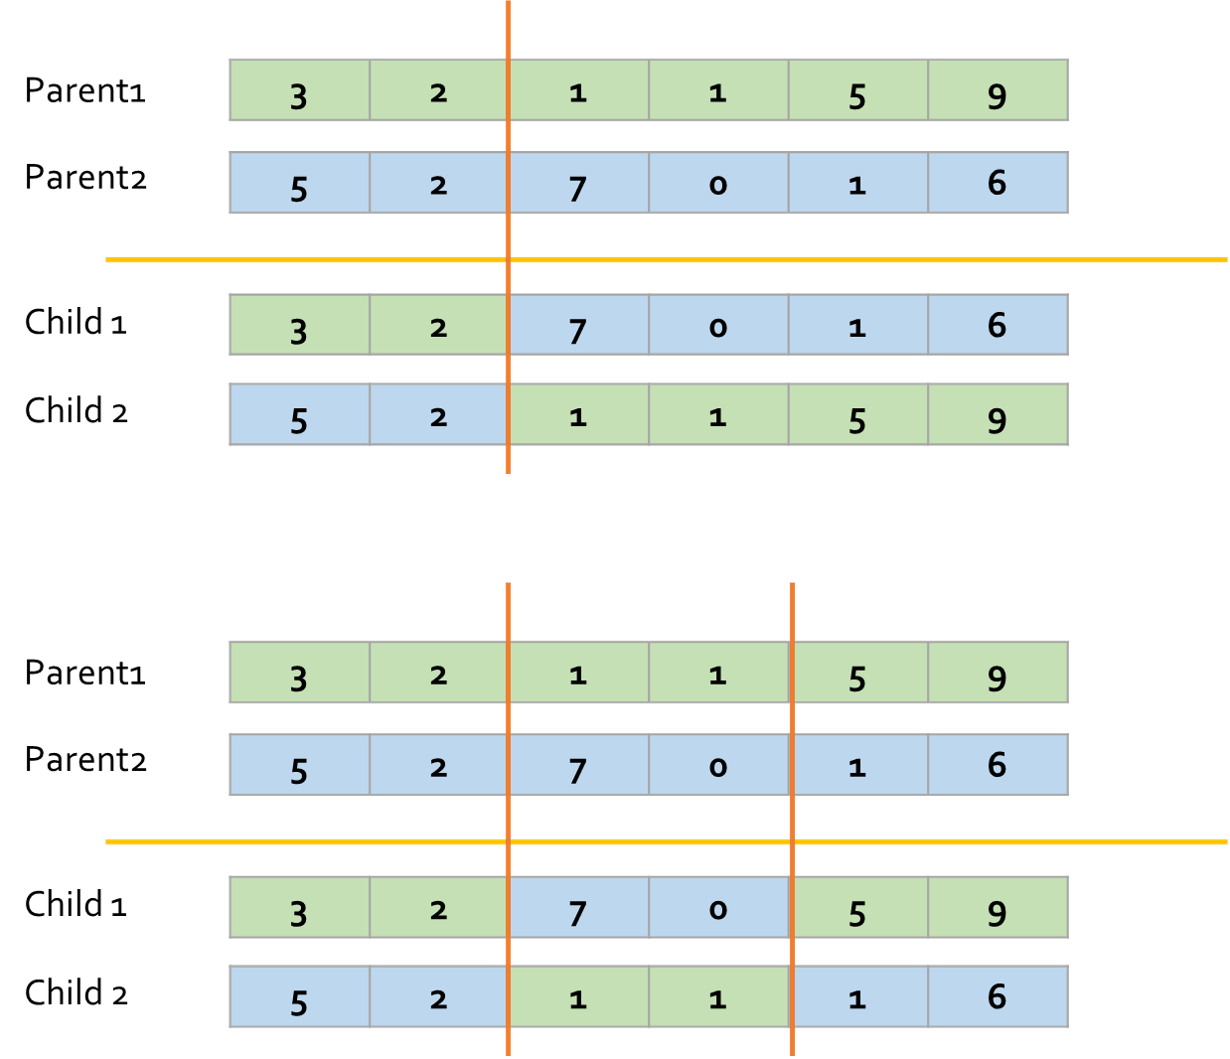
\includegraphics[width=0.8\textwidth]{img/crossover.png}
  \caption{Cruce de un punto (arriba) y cruce a dos puntos (abajo) aplicada a la mascara de individuos}
  \label{figure:crossover}
\end{figure}

\subsection{Operador de mutacion}
\label{subsection:mutation_operator}

La mutacion de los individuos de la poblacion ocurre solo al momento de hacer el
cruce de los mismos, es decir solo a los elementos nuevos se les aplica el
operador de mutacion, este operador puede modificar los siguientes elementos de
un individuo:
\begin{enumerate}
  \item La cantidad de piezas que conforman al individuo.
  \item El material del cual estan formados los elementos.
  \item El tipo de elemento que conforma a un individuo, es decir, modificar el
  valor del compuesto que forma parte del individuo.
  \item La posicion individual (\textit{x} o \textit{y}) de los compuestos.
\end{enumerate}

La manera en como se aplica el operador de mutacion se describe como sigue,
primero al momento de generar al nuevo individuo se realiza un calculo de
porcentaje en donde se decide si tendra o no mutacion dependiendo del procentaje
de mutacion que se haya asignado al inicio del algoritmo, posteriormente en caso
de que el valor de porcentaje quede dentro del rango se toma para las
operaciones, esta mismas se explican de la manera siguiente.

Para mutar la cantida de compuestos en un individuo primero se realiza una
seleccion aleatoria entre las opciones de agregar o quitar compuestos,
posteriormente en caso de requerir agregar mas se realiza una seleccion
aleatoria de entre la cantidad de compuestos creados, estos mismos se integran
al final de la lista de compuestos del individuo. Para eliminar elementos de la
lista se realiza una corrida por todos los elementos y en cada uno se realiza
una probabilida de \textit{50\%} de sea borrado de la lista, un ejemplo de este
proceso se muestra en la figura \ref{figure:mutate_add_remove} en donde se
presenta una tabla que denota las posiciones de los compuestos en base a la
mascara, en este ejemplo se realizo una corrida para remover elementos (color
rojo) y una segunda para agregar nuevos compuestos (color verde).

\begin{figure}
  \centering
  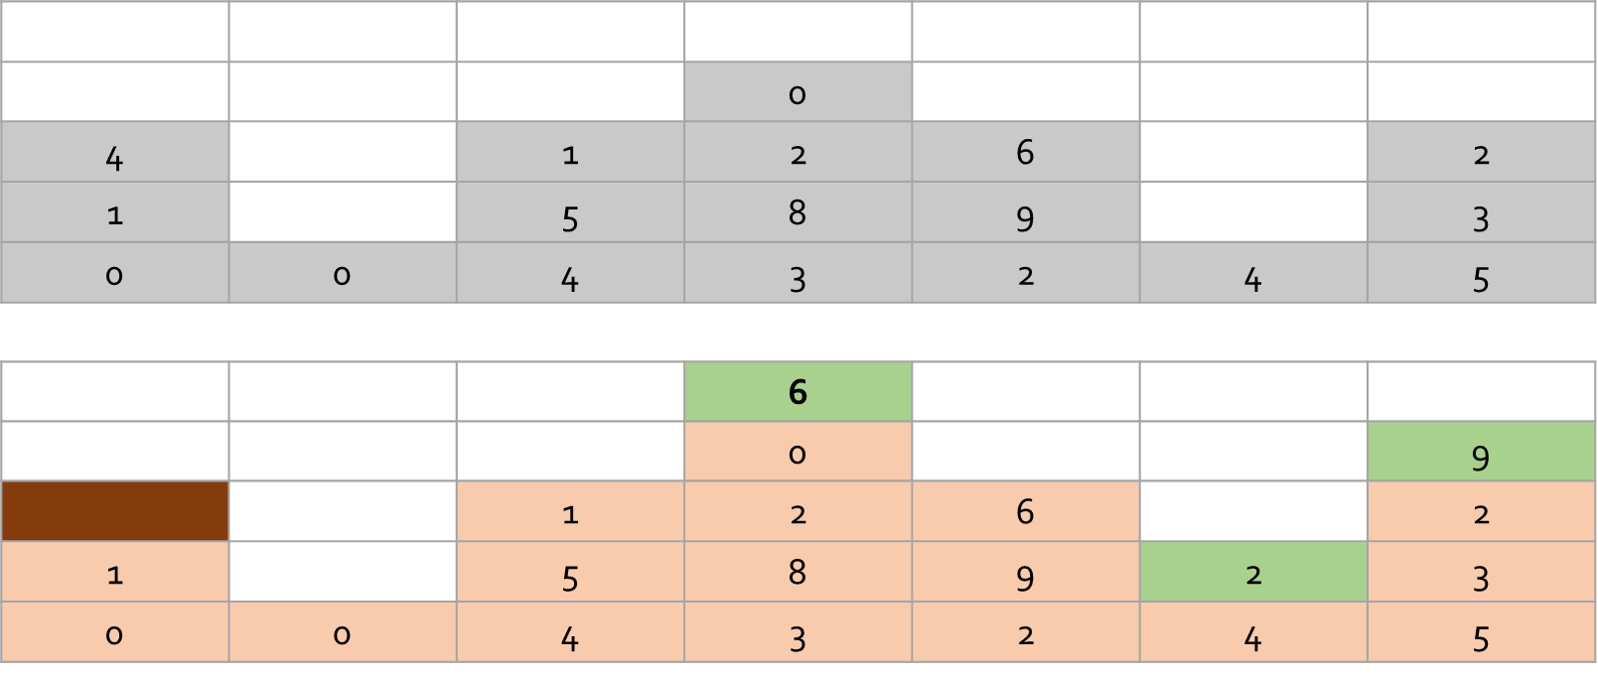
\includegraphics[width=0.85\textwidth]{img/mutation_add_remove.png}
  \caption{Ejemplo del operador de mutacion enfocado a remover y agregar compuestos}
  \label{figure:mutate_add_remove}
\end{figure}

La segunda mutacion se encarga de modificar el material del que estan
conformados los compuestos del individuo, la manera en como trabaja este proceso
es primero se selecciona aleatoriamente cuales compuestos seran modificados sin
repetir valores, posterioremente se modifica de manera aleatoria el valor que
define el tipo de material del que se conforma, para esto se toma en cuenta que
\textit{0} representa material de madera, \textit{1} representa material de
hielo y finalmente \textit{2} representa el material de piedra, debido a que el
juego solo acepta esta lista de compuestos no es posible asignar valores
diferentes a estos.

En la figura \ref{figure:mutate_material} se muestra un ejemplo de la manera en
como opera la mutacion del tipo de compuesto, en este ejemplo se muestra el
genotipo y fenotipo de un individuo, el genotipo muestra los colores naranja,
azul y gris para denotar los materiales de madera, hielo y piedra
respectivamente, en este caso la mutacion cambia el material de 5 elementos del
genotipo de madera a hielo, esto se refleja del lado derecho en donde se muestra
la vista actualizada del individuo despues de la mutacion.

Debido a que los compuestos generados pueden contener diferentes cantidades de
elementos en estos casos se cambia el material equitativamente a todos elementos
del compuesto, de esta manera se evita tener que realizar un recorrido por todo
el compuesto y mutar el material de cada uno.

\begin{figure}
  \centering
  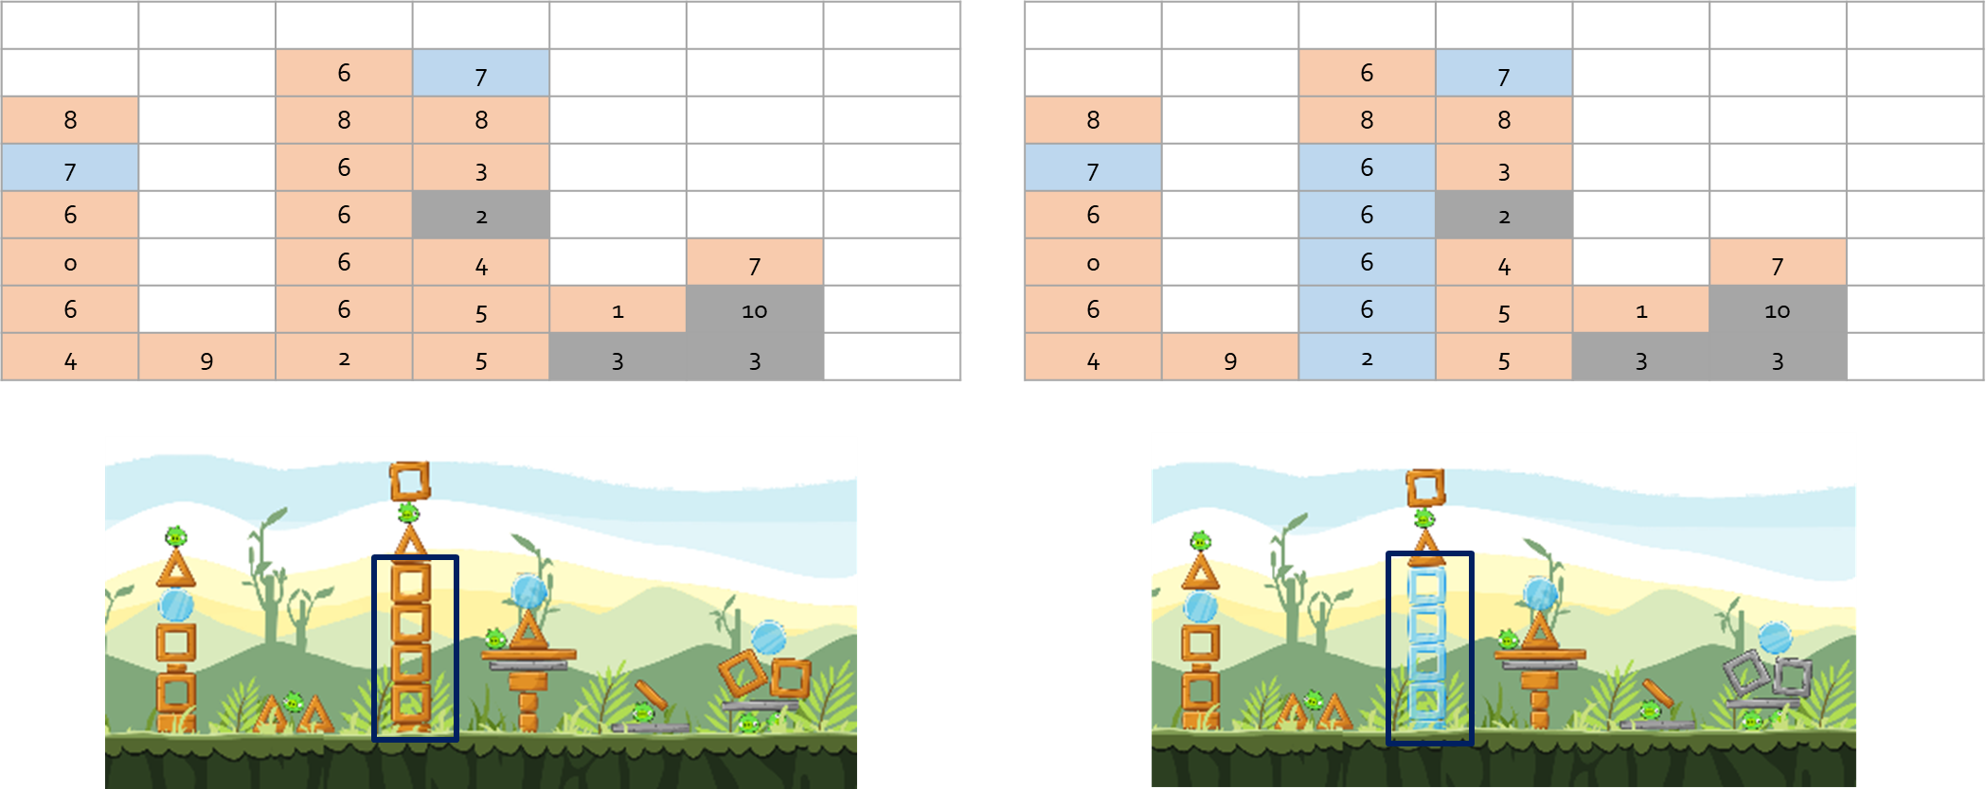
\includegraphics[width=0.95\textwidth]{img/mutation_material.png}
  \caption{Ejemplo del operador de mutacion enfocado a cambiar el material de los compuestos, pre-mutacion (izquierda) y post-mutacion (derecha)}
  \label{figure:mutate_material}
\end{figure}

La tercera mutacion se encarga de cambiar el compuesto que representa una
posicion del genotipo del individuo, este trabaja de una manera similar al
anterior en el sentido de que primero se selecciona a los individuos a mutar,
posteriormente a la seleccion se realiza una segunda seleccion aleatoria entre
las posiciones del genotipo del individuo, aquellos compuestos seleccionados son
cambiados por otro de la lista existente, para esto se realiza una seleccion de
un valor aleatorio que va desde \textit{0} hasta la cantidad de compuestos
existentes, por ejemplo suponiendo que se tiene solo la cantidad base de piezas
en el algoritmo entonces la seleccion sera un valor aleatorio desde \textit{0}
hasta \textit{10}.

La figura \ref{figure:mutate_composite} nos muestra un ejemplo de como es que
actua la mutacion de tipo de compuesto, en el ejemplo mostrado se tiene el
genotipo de un individuo combinado con su respectiva mascara asi como su
fenotipo respectivo (lado izquierda) al ser representado en la pantalla del
juego, en el lado derecho de la misma imagen se aprecia la modificacion de
compuestos realizada al genotipo base (marcado en amarillo), la modificacion de
compuestos en los individuos puede traer la conscuencia de que los niveles
generados sean inestables como en este ejemplo, esto a su vez puede permitir
identificar mascaras de los individuos que logran mantener la estabilidad de las
estructuras permitiendo asi mejorar el algoritmo.

\begin{figure}
  \centering
  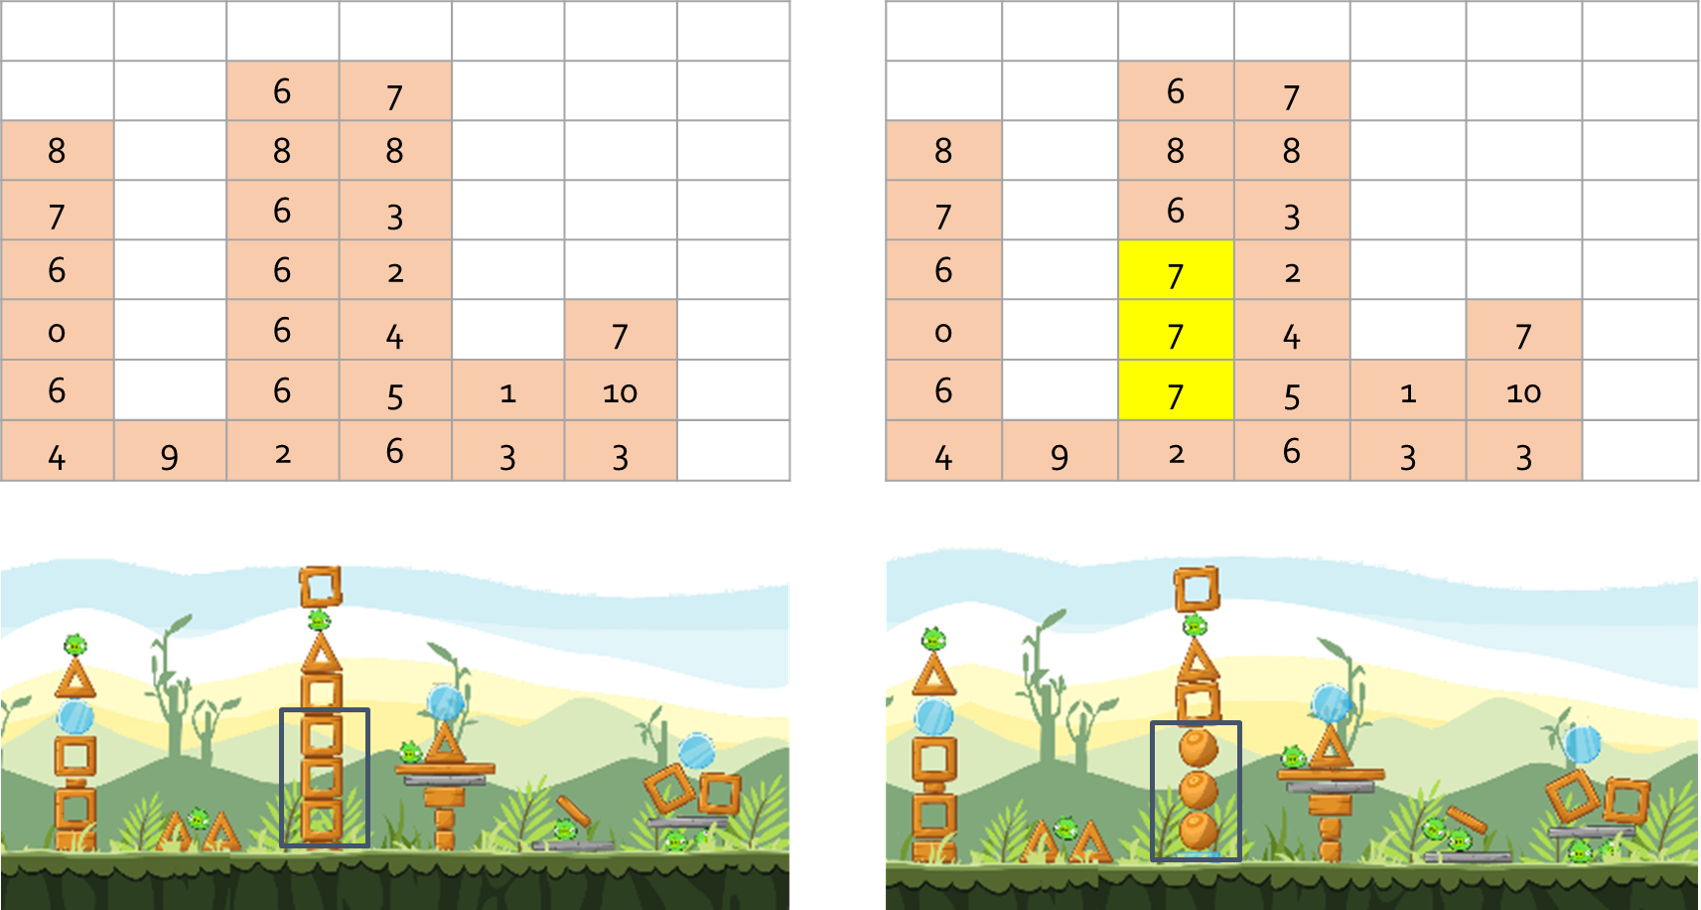
\includegraphics[width=0.9\textwidth]{img/mutation_composite.png}
  \caption{Ejemplo del operador de mutacion enfocado a cambiar los compuestos asignados, pre-mutacion (izquierda) y post-mutacion (derecha)}
  \label{figure:mutate_composite}
\end{figure}

El ultimo tipo de mutacion realizada en los individuos es la modificacion de las
posiciones \textit{x} y \textit{y} de algunos compuestos dentro del individuo,
la modificacion de las posiciones se realiza mediante una seleccion de valores
aleatorios de una distribucion gaussiana dentro de un cierto rango de distancia
para no permitir que los elementos se alejen demasiado de punto central
original.

\subsection{Representacion de individuos}
\label{section:individual_representation}

Una vez que se han agregado nuevos individuos a la poblacion, y que estos
individuos pasaron por su fase de mutacion si es que requerian se procede a
realizar la combinacion de los elementos que conforman al individuo con el fin
de generar los archivos requeridos para la simulacion de estos mismos, cabe
resaltar que esta combinacion se realiza tambien en los individuos iniciales
antes de la simulacion inicial, debido a que el juego requiere una
representacion mediante el uso de archivos en formatos \textit{XML}, se requiere
primero obtener la informacion de todos los elementos que conforman a un
individuo y posteriormente armar los archivos mediante el uso de estos datos.

\begin{figure}
  \centering
  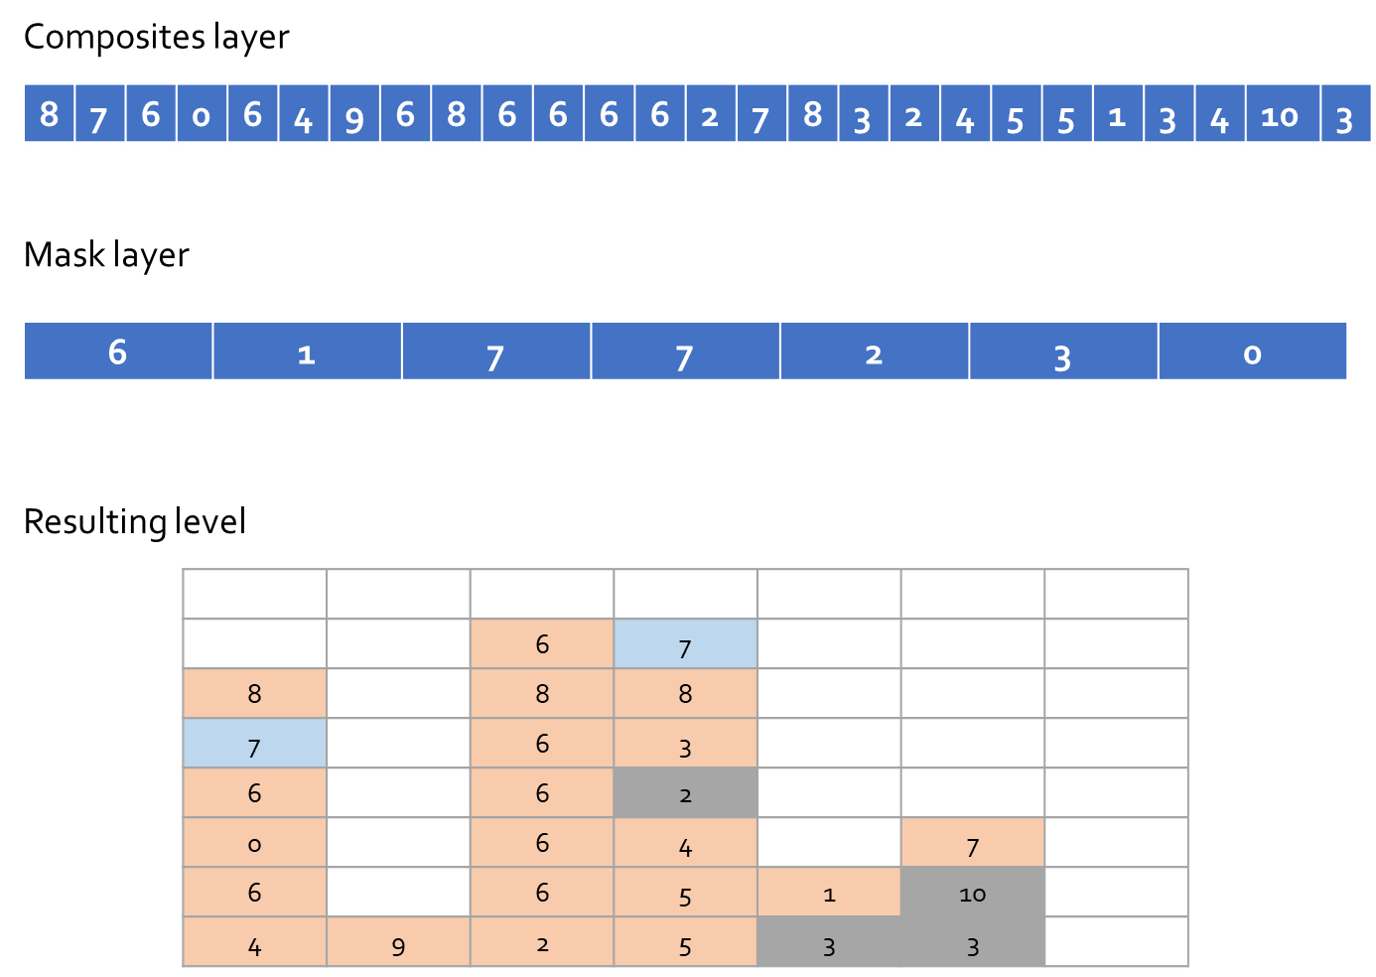
\includegraphics[width=0.9\textwidth]{img/layer12_combine.png}
  \caption{Ejemplo de la combinacion de capas de un individuo}
  \label{figure:individual_representation}
\end{figure}

En la figura \ref{figure:individual_representation} muestra la estructura de los
componentes de un individuo, un individuo es representado por \textit{2} capas
diferentes en forma de lista, la primera es la capa de compuestos, esta capa se
muestra la lista de compuestos que representan a un individuo, esta listas puede
variar en tamaño dependiendo de si durante las operaciones de mutacion se le
agregaron o quitaron elementos al individuo, de igual manera como se axplico en
el la seccion \ref{section:composite_creation} cada valor de la lista representa
no una pieza del juego sino uno de los compuestos que se crean antes de iniciar
el algoritmo o aquellos que se agregan durante el mismo en caso de haber.

La segunda parte que compone la representacion del individuo es la mascara, como
se explica en la seccion \ref{subsection:ruleofthirds} la idea detras del uso de
esta mascara es la de generar estructuras utilizando la lista de compuestos del
individuo, en esta misma seccion se presento una propuesta de crear mascaras en
donde se denotara la forma que se queria que tuviera un individuo particular,
aplicando estas estructuras en los individuos generaba los resultados esperados,
siendo el caso niveles en donde la distribucion de los compuestos crearan formas
diferentes como castillos, torres, casas o diferentes figuras, sin embargo
utilizar esta tipo de estructuras no permitia que el algoritmo lograra
evolucionar sino que simplemente encontraria la mejor combinacion de
piezas-mascara en determinado momento, por esto se opto por utilizar la
generacion de mascaras que se muestra en la figura
\ref{figure:individual_representation} y que fue explicado en la seccion
\ref{section:ind_generation} la cual unicamente muestra una determinada cantidad
de piezas a asignar en posiciones diferentes del nivel, esto permite tener mejor
diversidad en los individuos creados.

Al momento de combinar ambos componentes del individuo se obtiene un resultado
similar al mostrado en la parte inferior de la imagen en donde los compuestos se
organizan en manera de cola, es decir el primer elemento en la lista sera el
primero en ser colocado, una vez que se definen cuales elementos seran colocados
en cada columna el sistema calcula la altura total de cada compuesto y
comenzando desde la parte inferior coloca un compuesto en el nivel, despues
calcula la distancia desde la parte superior del mismo hasta la parte central
del siguiente para colocarlo de tal forma que al comenzar la simulacion no
aparescan en caida libre sino que aparescan una pieza sobre otra, de esta manera
se previenen problemas de balance al permitir que que las piezas caigan y
reboten en direcciones que provocaran que las estructuras terminen por caer
totalmente, en la misma imagen se aprecian cuadros de diferentes colores, estos
mismos representan el material del cual esta construido cada compuesto como se
explico en la seccion de mutacion anterior.

Finalmente una vez que se tiene la informacion anterior definida se procede a
realizar una busqueda de los lugares en donde apareceran los enemigos del juego,
la manera en como se define donde pueden aparecer estos es mediante una funcion
que revisa los compuestos que existen en el nivel, caundo un compuesto cumple
con ciertas caracteristicas se permite que uno de los enemigos pueda ser
colocado en la parte central o superiror del mismo, al iniciar este metodo se
busca aquellos que cumplen esta caracteristica y se ordenan en una lista
auxiliar, despues de manera pseudo-aleatoria se decide la cantidad de enemigos
que tendra el nivel, deacuerdo a este valor se seleccionan \textit{x} cantidad
de posiciones para colocar a los enemigos donde \textit{x} es el valor de
enemigos requeridos, una vez se definio en donde estaran colocados estos
enemigos se regresa una lista con las coordenadas \textit{x} y \textit{y} de las
mismas.

Mediante la combinacion de los enemigos con el genotico construido de un
individuo se obtiene el nivel a mostrar en el juego, una representacion de esto
se muestra en la figura \ref{figure:ind_representation_plus_pigs} en donde al
genotipo armado deacuerdo a los puntos anteriormente mencionados se le agrega el
listado de posiciones de los enemigos, en este caso los enemigos son
representados por un color verde en las posiciones en donde estaran, finalmente
esto permite tener la estructura de los niveles completa, esta informacion se
utiliza al momento de generar los archivos de \textit{XML} los cuales en el
software de simulacion generaran una vista de los mismos como se muestra en la
esquina inferior derecha de la misama imagen. 

\begin{figure}
  \centering
  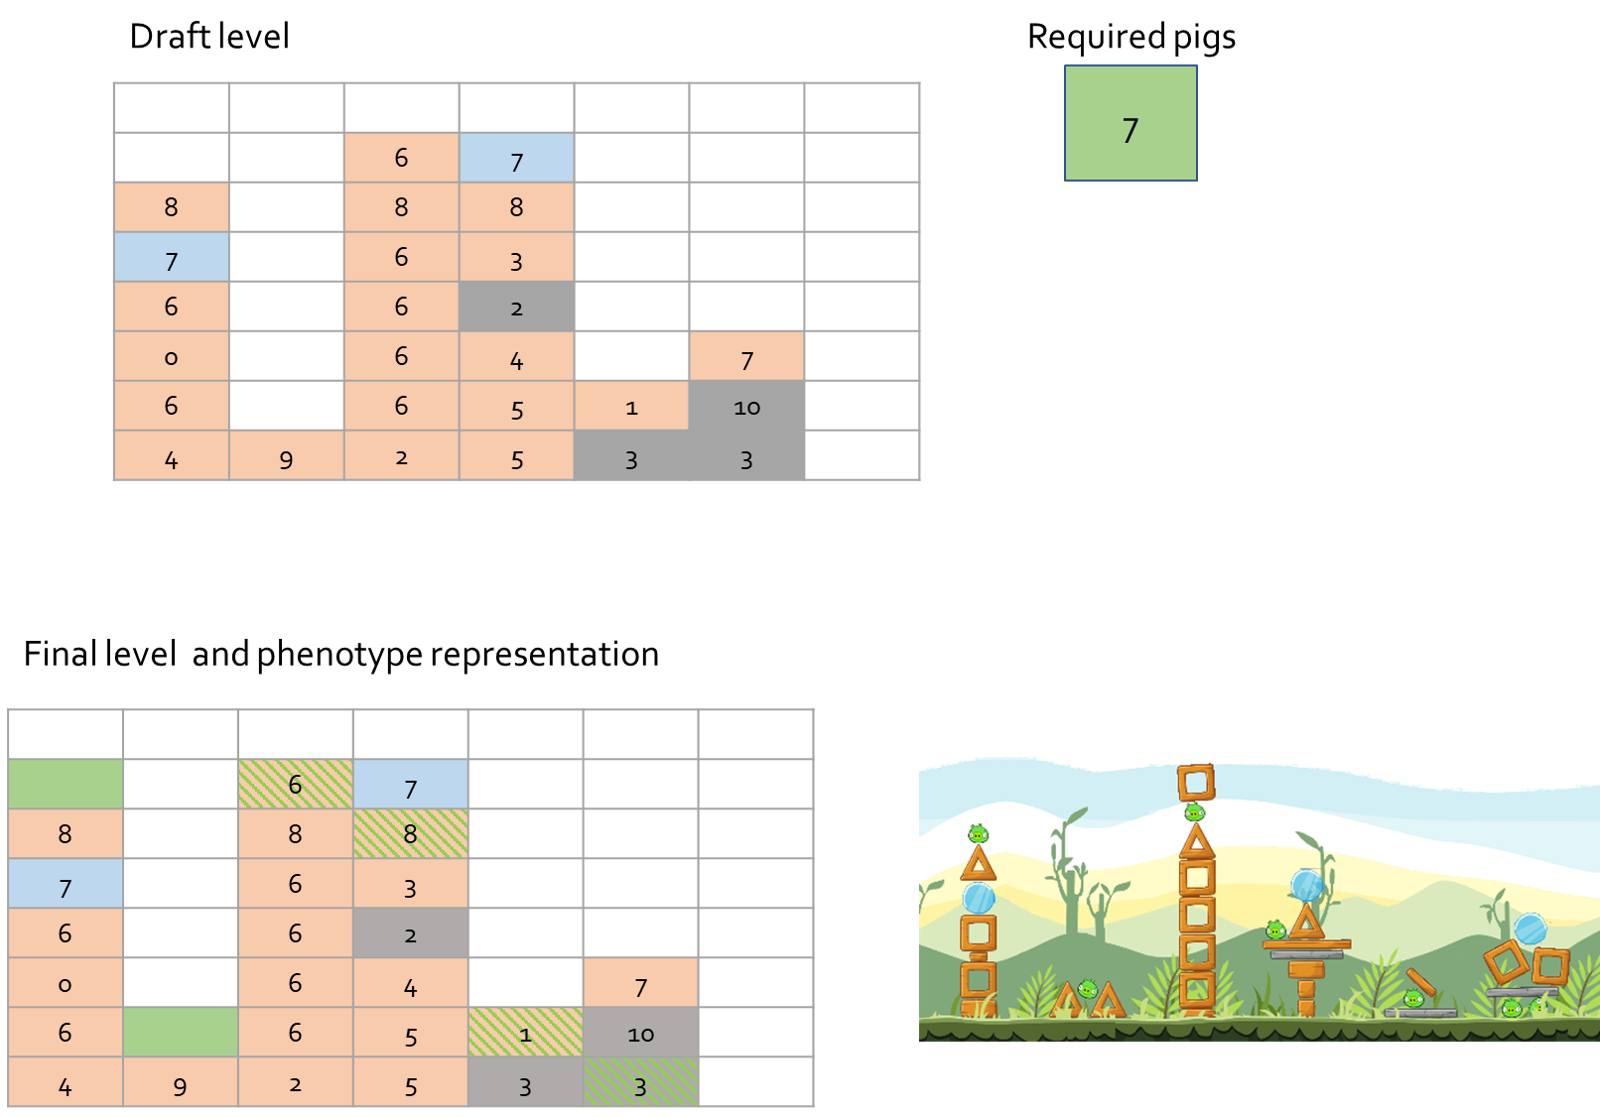
\includegraphics[width=0.9\textwidth]{img/layer123_combine.png}
  \caption{Ejemplo de la combinacion de un genotipo armado de la figura \ref{figure:individual_representation} con la colocacion de enemigos}
  \label{figure:ind_representation_plus_pigs}
\end{figure}

\subsection{Calculo de fitness}
\label{subsection:fitness_calculation}

Cuando los individuos pasan por el proceso de simulacion se genera un archivo en
formato \textit{XML} que contiene los resultados de los compuestos que fueron
puestos en los archivos antes de la simulacion con la diferencia de que estos
archivos contienen la informacion del ultimo estado de los mismos compuestos al
terminar dicha simulacion es decir se obtiene un listado de piezas y enemigos con
la informacion de sus posiciones \textit{x} y \textit{y} asi como del angulo con
en el cual quedaron al concluir la simulacion, ademas de esto se entrega la
informacion de la velocidad promedio de movimiento que tuvieron.

Esta informacion permite conocer las inperfecciones que tuvieron los nivles al
cuncluir las simulaciones, para mejorar la evaluacion obtenida que determina la
aptitud de los individuos se toma en cuenta una evaluacion de dos fases la
primera fase tiene que ver con la estabilidad de los individuos y se evalua en
base a dos metricas:
\begin{enumerate}
    \item La cantidad de piezas que no son destruidas durante la simulacion.
    \item Las posiciones finales de dichas piezas al terminar la simulacion.
\end{enumerate}

Para poder realizar el calculo de laspiezas presentes antes y despues de la
simulacion se utilizala informacion de las piezas anteriormente mencionada, sus
posiciones tanto \textit{x} como \textit{y} asi como del angulo de las mismas, a
esta informacion se le agrega un indicador de posicion para poder compararlo con
los datos del mismo indicador para las funciones siguientes, esta listado de
informacion se reraliza tambien antes de la simulacion con el fin de tener datos
con los cuales comparar, una vez que se tienen los datos se procede a realizar
el proceso de calculo de fitness, para calcular le diferencia de piezas se
compara la cantidad de elementos en ambas, debido que al momento de caer de
alturas grandes algunos elementos tienden a romperse entonces la cantidad de
elementos despues de la simulacion podra ser menor, para obtener el primer valor
se realizara un calculo para obtener un valor entre \textit{0} y \textit{100}
que define la calificacion en forma de porcentaje del total de piezas que se
salvaron en la simulacion es decir si antes de la simulacion se tenia un total
de \textit{10} piezas y al terminar la simulacion en el archivo correspondiente
solo existen \textit{5} entonces el individuo tendra una calificacion de
\textit{50\%} debido a que solo la mitad de las piezas no fueron destruidas.

El segundo valor toma se utiliza para definir si los conjuntos que no se
destruyeron se lograron mantener los mas estables posible, esto se calcula
mediante el uso de dos formulas mostradas en las formulas
\ref{equation:error_pos} y \ref{equation:error_ang} mediante el uso de estas
formulas se comprueba si las piezas se lograron o no mantener en sus posiciones
originales, en los casos donde las piezas no se hayan destruido se utilizan
estas formulas para revisar si las posiciones y angulos de inicio y final de la
simulacion son los mismos, en caso de que asi sea entonces no se realizan
modificaciones al fitness obtenido previamente, en caso contrario se obtiene una
penalizacion al fitness equivalente a una tercera parte del valor de porcentaje
por una pieza si se movio de posicion y otra tercera parte si su angulo cambio.

\begin{equation}
    \begin{split}
      error_{xy} = & 
      \begin{Bmatrix}
        0 \qquad si \qquad 0.08 > d \\ 
        \frac{100}{longitud\_piezas} * -0.33 \qquad si \qquad 0.08 < d
      \end{Bmatrix} \\
       d & = \sqrt{(x_2 - x_1)^2 + (y_2 - y_1)^2}
    \end{split}
    \label{equation:error_pos}
\end{equation}

\begin{equation}
    \begin{split}
      error_{r} = & 
      \begin{Bmatrix}
        0 \qquad si \qquad -5 < r < 5 \\ 
        \frac{100}{longitud\_piezas} * -0.33 \qquad si \qquad 0.08 < d
      \end{Bmatrix} \\
       r & = \left | rotacion_o \right | - \left | rotacion_f \right |
    \end{split}
    \label{equation:error_ang}
\end{equation}

Por otro lado la segunda fase de la evaluacion busca tener mas diversidad en los
individuos, esto es que tan \textit{nuevos} y \textit{diferentes} logran ser, la
manera en como se propone realizar esta evaluacion de diversidad es mediante el
uso de las metricas:
\begin{enumerate}
    \item La diversidad de las piezas utilizadas en el individuos
    \item El resultado de la funcion de entopia con las piezas utilizadas.
    \item La distancia \textit{Hamming} del mismo conjunto de piezas.
\end{enumerate}

Para evaluar la diversidad de los elementos primero se realiza un calculo de los
diferentes compuestos que integran a un individuo, para la evaluacion de esta
parte se toma en cuenta la diversidad que logra tener el indiviudo, en donde el
utilizar diferentes compuestos de la lista total permite tener una mejor
calificacion, esto es debido que mientras mas compuestos sean utilizados los
niveles que se pueden generar seran diversos entre si.

Posterior a esto se realiza un calculo de la entropia de un individuo, el
calculo de entropia es utilizado en la teoria de informacion para calcular el
nivele de desorden o incertidumbre en los individuos, la formula que se utiliza
para esto se muestra en \ref{equation:entropy}

\begin{equation}
  s = -\sum _{i} P_i log P_i
  \label{equation:entropy}
\end{equation}
\myequations{Ecuacion de entropia}

La manera en como la entropia es utilizada en este proyecto es para determinar
si un individuo se vuelve \textit{"aburrido"} o \textit{"interesante"} la manera
en como se define este concepto para el individuo es mediante la medicion de las
piezas semejantes en el mismo, deacuerdo a esto si la cantidad y tipos de
compuestos se repiten demasiado en el individuo entonces el individuo tiene
entropia baja o en otras palabras se vuelve \textit{"aburrido"} y
\textit{monotono}, es decir si se tiene entropia baja entonces significa que los
compuestos utilizados son mayormente iguales dentro del individuos los cual
generara un nivel demasiado simple a diferencia de si se tiene entropia alta
significa que la cantidad de compuestos diferentes es alta los cual generara
niveles con formas un poco mas impredecibles.

\begin{equation}
d = min \begin{Bmatrix} $ d(x, $ y)$ : $ x, $ y $ \epsilon $ C, si $ x \neq y $ entonces 1 $ sino $ 0 $ \end{Bmatrix}
\label{equation:hamming}
\end{equation}
\myequations{Ecuacion de la distancia Hamming}

Una vez que se obtuvo el calculo de la entropia del individuo se procede a
obtener la distancia \textit{Hamming} del mismo, de manera sencilla la
\textit{distancia de hamming} (Hamming distance en ingles) representa el calculo
realizado en dos cadenas de valores en donde el punto es encontrar el valor
minimo de sustituciones necesarias para cambiar una cadena a otra, visto de otra
manera, la \textit{distancia de hamming} se encarga de encontrar la distancia
mas corta entre dos cadenas, la manera en como funciona esta funcion se muestra
en la formula \ref{equation:hamming}, en esta misma ecuacion los objetos
\textit{x} y \textit{y} representan listas, en este caso se manejan listas de
valores boleanos es decir listas de valores \textit{0} y \textit{1}, una
explicacion mas simple se presenta en la funcion \ref{equation:hammin_example}.

\begin{equation}
  \begin{split}
    C = & \begin{Bmatrix} a, b, c \end{Bmatrix} \\
     & a = (00000) \\
     & b = (10110) \\
     & c = (01011) \\
     d(a, b) & = 3 \qquad d(a, c) = 3 \qquad d(b, c) = 4
  \end{split}
  \label{equation:hammin_example}
\end{equation}
\myequations{Ejemplo de uso de la distancia de Hamming}

\begin{equation}
  \begin{split}
    error_{r} = & 
    \begin{Bmatrix}
      0 \qquad si \qquad -5 < r < 5 \\ 
      \frac{100}{longitud\_piezas} * 0.5 \qquad si \qquad 0.08 < d
    \end{Bmatrix} \\
     r & = \left | rotacion_o \right | - \left | rotacion_f \right |
    % d(a, b) & = 3 \qquad d(a, c) = 3 \qquad d(b, c) = 4
  \end{split}
  \label{equation:error_ang}
\end{equation}

En esta funcion se tiene un conjunto de listas representado por \textit{C}, en
este conjunto existen las listas \textit{a, b y c}, para poder encontrar la
\textit{distancia de hamming} de cada par de listas se utiliza la formula
\ref{equation:hamming} esto es, se revisa cada par de elementos de la listas y
se suma \textit{1} si los elementos son diferentes, de esta manera se logra
determinar que la cantidad de cambios necesarios para hacer que la lista
\textit{b} se asemeje completamente a la lista \textit{a} es \textit{3} debido a
que solo se requiere cambiar los tres valores \textit{1} en la lista \textit{b},
la razon por la que no es requerido cambiar valores en la lista \textit{a} es
debido a que en la funcion la segunda lista utilizada es la que se quiere
asemejar a la primera no solamente cambiar una lista a otra.

Al utilizar la distancia de \textit{hamming} se obtiene como mencionado
anteriormente la cantidad menor de cambios para asemejar una lista a otra, sin
embargo como el fin de sistema es crear niveles que sean diferentes entre si
entonces es posible incluso modificar la evaluacion para obtener este valor para
obtener la mayor distancia posible de tal modo que se sabra cuales individuos
tendran la tendencia de ser diferentes para generar mas diversidad.

\subsection{Seleccion de miembros elite}
\label{subsection:elite_selection}

Finalmente despues de obtener los resultados de aptitud de los individuos se
procede a realizar la seleccion de aquellos que lograran integrar el grupo de
elite que se utilizara para sustituir miembros de la poblacion al inicio de la
siguiente generacion, para realizar esto primero se requiere ordenar todos los
individuos por medio de su respectivo valor de fitness desde el valor mas alto
hasta el valor mas bajo, posteriormente se toma una determinada cantidad de
individuos iniciando desde el mejor, la cantidad de individuos que se tomaran
para el grupo de elite es una cantidad que se define antes de iniciar el
algoritmo genetico.

Una vez que se ah tomado la cantidad de individuos requerida se procede a
integrar estos mismos individuos a el grupo de elite, para realizar la
integracion al grupo de elite primero se requiere analizar el estado del grupo,
en caso de que no existan elementos en la lista lo cual solo sucede en la
primera generacion, el grupo seleccionado se integra automaticamente a la lista
de elite, despues se ordena la lista deacuerdo al valor de aptitud y se corta de
tal manera que la lognitud de la lista de elite sea menor o igual a un valor que
se determina antes de iniciar el algoritmo, en caso de que ya existan elementos
en el grupo entonces estos miembros se integran al final de la lista del grupo
elite, se realiza un reordenamiento en la lista en base al valor de aptitud de
los individuos y se corta la lista en caso se ser requerido.

Una vez que se han completado todos los procesos anteriormente explicados el
algoritmo agrega datos de los mejores, los perores y el promedio de los valores
de aptitud de los individuos en listas que sirven para realizar promedios al
final de toda la ejecucion del codigo, ademas de esto tambien se guarda
informacion de los resultados individuales de las funciones de \textit{entropia}
y la \textit{distancia de hamming} con el fin de ver en manera de graficas el
comportamiento del algoritmo bajo los datos que le fueron proveidos al inicio de
la ejecucion. Al terminar este proceso de integracion de datos se realiza el
ultimo movimiento en la informacion de la generacion siendo este obtenerlos
archivos \textit{XML} de los individuos y guardandolos en una nueva locacion con
el fin de mantener un registro del progreso de los individuos durante la
ejecucion del algoritmo.